\section{The discontinuous Galerkin spectral element method (DGSEM)\label{sec:dgsem}}
CMT-nek solves Equation~\ref{claw} by partitioning the
domain $\Omega \subset \mathbb{R}^d$, $d={1,2,3}$  into nelt non-overlapping elements (Figure~\ref{elements}),
the $e$\textsuperscript{th} of which is $\Omega_e$,
and marching the left-hand-side of Equation~\ref{claw} forward in time on
each element. The right-hand-side of Equation~\ref{claw} is discretized on
each element in a very peculiar way called \textbf{the two-point form of DGSEM}
that is only briefly summarized here.
The two-point form of DGSEM brings discontinuous Galerkin methods and finite
difference methods together in a very peculiar way, and the reader is strongly encouraged to study the bibliography carefully.

\subsection{Weighted residuals\label{sec:wrt}}
Galerkin methods force an inner product of Equation~\ref{claw} with a test function to vanish
for every value of the test function in some basis spanning a finite-dimensional
space of test functions $\chi$.
Integrating this inner product by parts on a given element$\Omega_e$ gives us the \textbf{weak form} of the discontinuous Galerkin weighted residual
statement for the governing equation~\ref{claw}:
\begin{equation}
\int_{\Omega_e} v(\bx) \pp{\bU(\bx)}{t}dV = 
\int_{\Omega_e} \left(\nabla v\right) \cdot \bH\, dV  
-\int_{\dO_e} v(\bx) \bH^{\ast}(\bU^-,\bU^+) \cdot \bhn dA +
\int_{\Omega_e} \mathbf{R}(\bx) v(\bx) dV,
\label{dghweak}
\end{equation}
where the surface integral term $\bH\cdot\bhn$ in the surface integral has been replaced by
the \textbf{numerical flux} $\bH^{\ast}(\bU^-,\bU^+)\cdot \bhn$ that, since $\chi$
is a broken space defined on each element, resolves the discontinuities between
the representation of $\bU$ on the faces of $\Omega_e$ and the corresponding $\bU$
in the neighbors sharing faces $f \in \dO_e$. That is,
\begin{align}
   U^-(\bx) \equiv & U(\bx) \mbox{ taken from the \textbf{interior}, or trace, of }\Omega_e \label{uminus}\\
   U^+(\bx) \equiv & U(\bx) \mbox{ taken from the \textbf{element adjacent to} }\Omega_e\mbox{ sharing }\dO_e. \label{uplus}
\end{align}
The numerical flux functon $\bH^{\ast}$ is critically important to the stability
and convergence properties of DGSEM, and will be presented in more detail in
\S\ref{}.

\begin{figure}
\centering
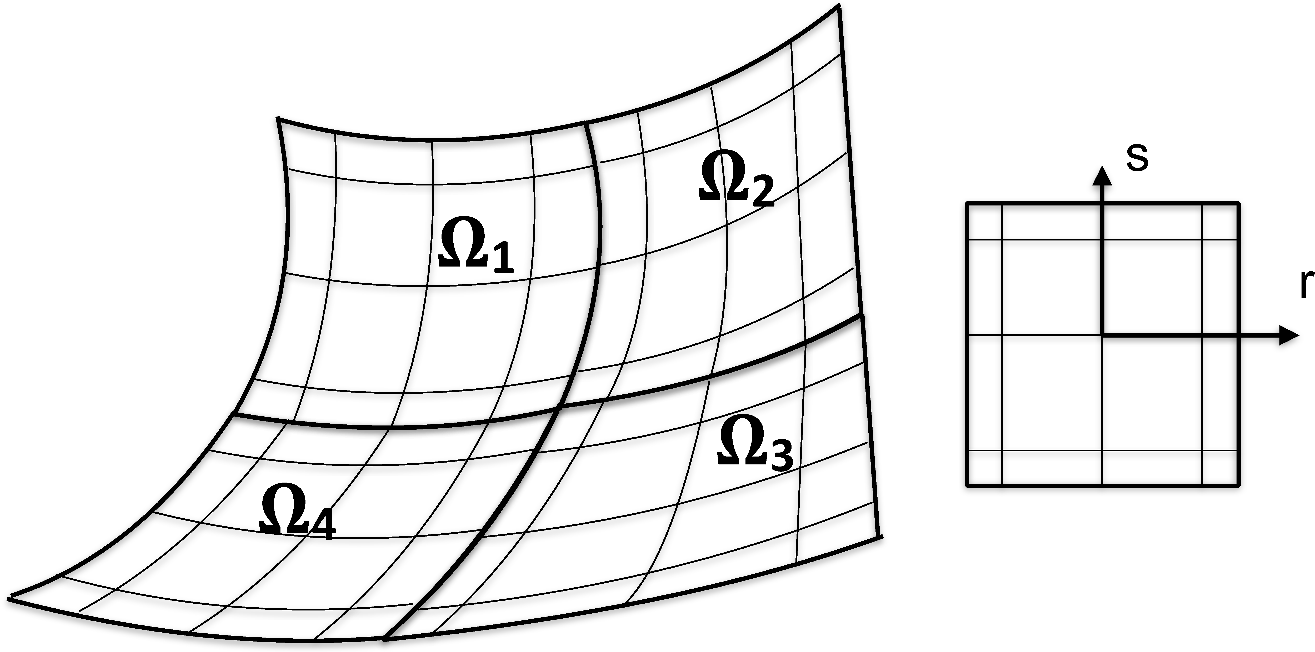
\includegraphics[width=8.0cm]{elements}
\caption{A schematic representation of spectral elements and the reference element in two dimensions.}
\label{elements}
\end{figure}

Figure~\ref{elements} also illustrates how a point $\bx\in\Omega_e$ is isoparametrically mapped to
$\mathbf{r}\equiv\left(r,s,t\right)^{\Txp}=\left(r_1,r_2,r_3\right)^{\Txp}$ in the reference element
$\Oh=[-1,1]^3$,
This transformation has, $\forall \mathbf{x}\in\Omega_e$,
Jacobian $J(\mathbf{x})\equiv|\partial \mathbf{x}/\partial \mathbf{r}|$ and
metrics $\partial r_i/\partial x_j$.

We integrate the right-hand-side (RHS) of Equation~\ref{dghweak} by parts a second time to get
the \textbf{``strong'' form} of the weighted residual statement,
\begin{equation}
\int_{\Omega_e} v(\bx) \pp{\bU(\bx)}{t}dV = 
\int_{\Omega_e} v \nabla \cdot \bH\, dV  
-\int_{\dO_e} v(\bx) \left(\bH-\bH^{\ast}\right) \cdot \bhn dA +
\int_{\Omega_e} \mathbf{R}(\bx) v(\bx) dV.
\label{dghstrong}
\end{equation}
The distinction between weak and strong forms is ultimately unimportant in DGSEM,
but strong form (Equation~\ref{dghstrong}) is clearer and more convenient.

\subsection{Quadrature and approximation}
All integrals in Equation~\ref{dghstrong} are now approximated by
\textbf{Gaussian quadrature}, as described in \S whatever of \cite{dfm02}.
We evaluate the solution $\bU$ and various functions of it (like fluxes $\bH$ and
source terms $\mathbf{R}$) on a grid of $N^3$ \textbf{Gaussian quadrature nodes}
within each element. This means:
\begin{enumerate}
\item The approximation space $\chi$ becomes $[\mathbb{P}^{N-1}]^3$, a Cartesian product of the space of all
polynomials of degree $N-1$.
\item The basis functions are a \textbf{nested tensor product} of the \textbf{interpolating Lagrange
polynomials} evaluated on $N^2$ lines of $N$ Gaussian quadrature nodes. This is
described in more detail in \S of \cite{dfm02}.
\item The discrete unknowns are the \textbf{nodal values} $\bU(x_i,y_j,z_k)$ at each of the $N^3$ Gaussian nodes in each element.
\end{enumerate}
Finally, within the family of Gaussian quadrature we specifically choose the
\textbf{Gauss-Legendre-Lobatto (GLL)} nodes. Formulas for $\omega$ and $\mathbf{r}$ may be found in Appendix of \cite{dfm02}.

Nodal values at grid points within a given element are arranged into
vectors lexicographically:
\begin{equation}
\mathbf{u}\equiv\left[\begin{array}{c} U(x_1,y_1,z_1) \\  U(x_2,y_1,z_1) \\ \vdots \\ U(x_N,y_N,z_N) \end{array}\right],
\mathbf{v}\equiv\left[\begin{array}{c} v(x_1,y_1,z_1) \\ v(x_2,y_1,z_1) \\  \vdots \\ v(x_N,y_N,z_N) \end{array}\right],
\mathbf{h}_1\equiv\left[\begin{array}{c} H_x(U(x_1,y_1,z_1))\\ H_x(U(x_2,y_1,z_1))\\   \vdots \\ H_x(U(x_N,y_N,z_N)) \end{array}\right],
\label{gridvects}
\end{equation}
with $u_l=U(x_i,y_j,z_k)$ when $l=i+N(j\!-\!1)+N^2(k\!-\!1)$.

These vectors may be catenated one element after the other into a vector $\buu_L$ of $N^3 K$ nodal
values for
the quadrature nodes in the entire mesh.

To assist notation for scalar multiplication, we introduce the diagonal matrix formed
from an arbitrary nodal vector $\mathbf{f}$
\begin{equation}
\mbox{diag}(\mathbf{f})\equiv \left[\begin{array}{cccc} f(x_1,y_1,z_1) & & & 0 \\
                                                        & \diagdown & & \\ 
                                                        & & f(x_i,y_j,z_k)  & \\
                                                        & & \diagdown & \\
                                                        & & & \\
                                                        0 & & & f(x_N,y_N,z_N)\end{array}\right].
\label{diagalot}
\end{equation}

Consider the left-hand-side of Equation~\ref{dghstrong}. Approximating everything with
the nodal representation on $N^3$ GLL points described above,
means our discrete equation becomes, at the top level,
\begin{equation}
\int_{\Omega_e} v(\bx) \pp{\bU(\bx)}{t}dV \approx \bv^{\Txp}\mathbf{B}\pp{\bu}{t} =
\mbox{RHS},
\label{firstdiscrete}
\end{equation}
where RHS is the right-hand-side of Equation~\ref{dghstrong}
evaluated at each GLL node. Bold-faced quantities are nodal vectors (Equation~\ref{gridvects}) including
the mass matrix $\mathbf{B}$,
\begin{equation}
\mathbf{B}\equiv \left[\begin{array}{ccc} \diagdown & & 0 \\ &  \omega_i\omega_j\omega_k J(\mathbf{x}(r_i,s_j,t_k)) &  \\  0 & & \diagdown \end{array}\right],
\label{masslex}
\end{equation}
where $\omega_i$ is the GLL quadrature weight associated with the $i$\nth quadrature
node,
and $J_e(\mathbf{x})$ is the Jacobian $J$ of the mesh transformation described
above at the GLL points within $\Omega_e$.

The Galerkin statement is enforced for all possible test functions in $\chi$ by
equating coefficients of the test function $\mathbf{v}$ on both sides of Equation~\ref{firstdiscrete}.
%\textbf{It suffices for me to state that
%any operation in the volume integral in Equation~\ref{dghstrong} using the transpose
%of a matrix or a Kronecker product labeled as a transpose is really being applied to the test functions.}
Further multiplication of Equation~\ref{firstdiscrete} by $\mathbf{B}^{-1}$ produces the semidiscrete method of lines
\begin{equation}
\pp{\bu}{t} =\mathbf{B}^{-1}\mbox{RHS}=I_{\mbox{vol}}-I_{\mbox{sfc}},
\label{dgsemifinal}
\end{equation}
which may be integrated in time to solve for the nodal values $\bu$ of the conserved variables.
Right-hand-side terms in Equation~\ref{dgsemifinal} are essentially the effects
contributions of individual GLL nodes to integrals (hence the ``I''
abbreviation). We describe those in the following section.
